
\begin{figure}[H]
	\centering
	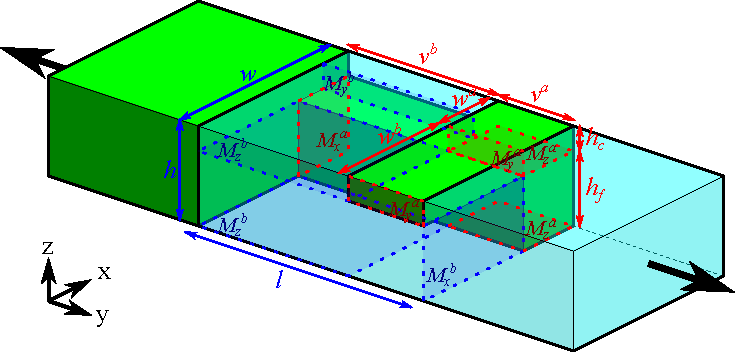
\includegraphics[width=\columnwidth]{sources/method/straight_model_v3.pdf}
	\caption{
		One straight unit cell connecting material $a$ (left) to material $b$ (right).
		Failure can happen along the fingers ($M_x$), along the cross beams ($M_y$) or at the interface between the two ($M_z$) for either material.}
	\label{fig:failure_modes}
\end{figure}


\section{Straight design}

\iffalse
The bending constraint is given by:
\begin{align*}
	\sigma_\text{max} &= \frac{M}{I}c \\
	c &= \nicefrac12 h \\
	I &= \frac{b h^3}{12} \\
	M &= \frac{w L^2}{8} \\
	w &= \frac{F}{L} \\
	\sigma_\text{max} &= \frac{12 F L}{8 b h^3} \nicefrac12 h \\
	\sigma_\text{max} &= \frac{3 F L}{4 b h^3} h \\
	\sigma_\text{max} &= \frac{3 F L}{4 b h^2} \\
\end{align*}
\fi


\Cref{fig:failure_modes} shows one cell of the straight structure, along with the design variables and the failure modes.
The optimization then consists of the following:

\begin{align}
	& \omit\rlap{$\displaystyle \max{ \frac{F}{\left( w^a + w^b \right) \left( h_\text{f} + h_\text{c} \right) }}$} \label{eq:obj} \\
% 	& \min{ h_\text{f} + h_\text{c}}
\omit\rlap{subject to} \nonumber \\
	w^m &\ge 2 w_\text{min}^m 								&&\text{ Nozzle size} \label{eq:c1} \\
	v^m &\ge w_\text{min}^m 								&&\text{ Nozzle size}  \label{eq:c2} \\
	h_\text{f} &\ge h_\text{min}  							&&\text{ Layer thickness}  \label{eq:c3} \\
	h_\text{c} &\ge h_\text{min} 							&&\text{ Layer thickness}  \label{eq:c4} \\
	v^a + v^b &\le l_\text{max} 							&&\text{ Design constraint}   \label{eq:c_total_length} \\
	\frac{ F }{ w^m h_\text{f} } &\le \sigma^m_\text{fail} &&\text{ Tension failure } M_x^m  \label{eq:c_tensile} \\
	\frac{ 3 F }{ 4 v^m h_\text{c}} &\le \nicefrac12 \sigma^m_\text{fail} 			&&\text{ Shear failure } M_y^m  \label{eq:c_shear} \\
	\frac{ 3 F }{ 4 v^m w^m } &\le \tau^m_\text{Z} 			&&\text{ Shear failure } M_z^m  \label{eq:c_shear_z} \\
	\frac{ 3 F w^b }{ 4 \left( v^a \right)^2 h_\text{c} } &\le \sigma^a_\text{fail}			&&\text{ Bending failure } M_y^a  \label{eq:c_bending_a} \\
	\frac{ 3 F w^a }{ 4 \left( v^b \right)^2 h_\text{c} } &\le \sigma^b_\text{fail}			&&\text{ Bending failure } M_y^b  \label{eq:c_bending_b} \\
	& \text{for both materials } && m \in \{a, b\} \nonumber
\end{align}

This looks like a multi-objective optimization problem, but without the second objective the problem is under-constrained.
Adding the second objective actually means there's one unique solution - rather counter-intuitively.

The $v^m$ variables don't figure in the objective, but they do appear in the constraints and therefore are also subject to the optimization.

Under different circumstances the values of the constraints will be different.
Because of manufacturing constraints we know that the layer thickness has to be smaller than half the smallest nozzle size:
$h_\text{min} < \nicefrac{1}{2} w^m_\text{min}$.
Depending on the design we might apply a different $l_\text{max}$, 
but it is required that $l_\text{max} \ge v_\text{min}^a + v_\text{min}^b$.
Materials properties of 3D printed materials are always such that $\tau_Z^m < \tau^m$.
Maximum shear stress theory further gives us that $\tau^m = \nicefrac12 \sigma^m_\text{fail}$.

Can we perhaps derive the something like following?
\begin{align*}
	\frac{ 3 F }{ 4 v^m h_\text{c}} &\le \tau^m 	\\
%	<? \frac{ 3 F }{ 4 v^m w^m } &\le \tau^m_\text{Z} 	\\
	<? \frac{ F }{ w^m h_\text{f} } &\le \sigma^m_\text{fail}
\end{align*}

Conversely, if $\nicefrac{w^b}{v^a} > \nicefrac{ \sigma^a_\text{fail} }{ \tau^a } = 2$ 
then the shear failure constraint \cref{eq:c_shear} is dominated by the bending failure constraint \cref{eq:c_bending_a},
since then 
$
\frac{ 3 F w^b }{ 4 \left( v^a \right)^2 h_\text{c} \sigma^a_\text{fail}}
> \frac{ 3 F }{ 4 v^a h_\text{c} \tau^a} 
$.
Otherwise the latter is dominated by the former.
The same holds conversely with the materials $a$ and $b$ swapped.
Therefore two of \cref{eq:c_shear}, \cref{eq:c_bending_a} and \cref{eq:c_bending_b} will be redundant.


Depending on the types of material used the tensile and shear strength in the Z direction can be an order of magnitude lower than in the horizontal directions.
In such a case the Z shearing failure constraint \cref{eq:c_shear_z} will be active for that material.

Suppose that \cref{eq:c_shear_z} is active.
\tim{Some steps?}
So we can conclude that \cref{eq:c_shear_z} is not active.

So some combination of \cref{eq:c_tensile,eq:c1} needs to be active on $a$ and $b$. 
\tim{Some steps?}
So \cref{eq:c1} is active on material $a$, and \cref{eq:c_tensile} is active on both material $a$ and $b$.


If \cref{eq:c_tensile} is active and \cref{eq:c_shear} is active then we can show that we can choose the height values such that \cref{eq:c_shear_z} is not active.

If \cref{eq:c_tensile} is active and \cref{eq:c_shear} is not active then?




\subsection{Monotonicity Analysis}
\tim{TODO: Convert objective function into a minimization problem and flip the signs everywhere.}
\begin{align*}
	\max{ \frac{F}{\left( w^a + w^b \right) \left( h_\text{f} + h_\text{c} \right) } }
																		&& F^+, w^{a-}, w^{b-},  h_\text{f}^-, h_\text{c}^-\\
\omit\rlap{subject to} \nonumber \\
	1 - \nicefrac{w^m }{2 w_\text{min}^m} &\le 0    							&& w^{m-} \\
	1 - \nicefrac{v^m }{w_\text{min}^m} &\le 0    							&& v^{m-} \\
	1 - \nicefrac{h_\text{f}}{h_\text{min}} &\le 0 							&& h_\text{f}^- \\
	1 - \nicefrac{h_\text{c}}{h_\text{min}} &\le 0 							&& h_\text{c}^- \\
	\frac{v^a + v^b}{ l_\text{max} }  - 1&\le 0 						&& v^{a+}, v^{b+} \\
	\frac{ F }{ w^m h_\text{f} \sigma^m_\text{fail} } - 1&\le 0 		&& F^+, w^{m-}, h_\text{f}^- \\
	\frac{ 3 F }{ 4 v^m h_\text{c} \tau^m } - 1 &\le 0 					&& F^+, v^{m-}, h_\text{c}^- \\
	\frac{ 3 F }{ 4 v^m w^m \tau^m_\text{Z} } - 1 &\le 0 				&& F^+, v^{m-}, w^{m-} \\
	\frac{ 3 F w^b }{ 4 \left( v^a \right)^2 h_\text{c} \sigma^a_\text{fail} } - 1 &\le 0			&& F^+, w^{b+}, v^{a-}, h_\text{c}^-\\
	\frac{ 3 F w^a }{ 4 \left( v^b \right)^2 h_\text{c} \sigma^b_\text{fail} } - 1 &\le 0			&& F^+, w^{a+}, v^{b-}, h_\text{c}^-\\
	& \text{for both materials } && m \in \{a, b\}
\end{align*}

If we would scale all design variables linearly with some factor $R$ and $F$ by $R^2$ then the objective function and all mechanical constraints \crefrange{eq:c_tensile}{eq:c_bending_b} remain at the same value.
If only those constraints were to be considered the problem would have been under-constrained.
Therefore some of the constraints \crefrange{eq:c1}{eq:c_total_length} will have to be active.
%incorrect! : Since only \cref{eq:c_total_length} provides an upper bound it must be active.
If we set \cref{eq:c1} active for material $a$ \todo{we will show} that none of the other constraints will be violated, so this constraint has to be active.

Let's assume \cref{eq:c_shear_z} is inactive.
In that case the objective function value and all the mechanical constraint values are invariant under scaling of $F$, $h_\text{f}$ and $h_\text{c}$ by any value $R$.
Therefore, either constraint \crefrange{eq:c1}{eq:c2} needs to be active.
We will assume that \cref{eq:c1} is active and \todo{we will show} that this doesn't violate \cref{eq:c2},
thus showing that the assumption is correct.


Let's \todo{assume} that \cref{eq:c_tensile} is active for both materials.
We can then derive:
\begin{align*}
%	\frac{ F }{ w^a h_\text{f} } &= \sigma^a_\text{fail} \\
%	\frac{ F }{ w^b h_\text{f} } &= \sigma^b_\text{fail} \\
%	\frac{ \nicefrac{ F }{ w^a h_\text{f} } }{ \nicefrac{ F }{ w^b h_\text{f} } } &= \frac{w^b}{w^a} = \frac{ \sigma^a_\text{fail}}{\sigma^b_\text{fail}} \\
	w^b &= w^a \frac{ \sigma^a_\text{fail}}{\sigma^b_\text{fail}} 
\end{align*}



The $v^m$ variables will have to be decided on by one of \crefrange{eq:c_shear}{eq:c_bending_b}.
Let's \todo{assume} that \cref{eq:c_shear} is active for material $b$.
We can then derive:
\begin{align*}
 	%\frac{ 3 F }{ 4 v^b h_\text{c}} &= \tau^b
	%\frac{ 3 F }{ 4 v^b h_\text{c}} &= \frac12 \sigma^m_\text{fail} \\
	%\frac{ F }{ w^b h_\text{f} } &= \sigma^m_\text{fail} \\
	\frac{ F }{ 2 w^b h_\text{f} } &= \frac{ 3 F }{ 4 v^b h_\text{c}} \\
	\frac{ 1 }{ 2 w^b h_\text{f} } &= \frac{ 3 }{ 4 v^b h_\text{c}} \\
	4 v^b h_\text{c} &= 6 w^b h_\text{f} \\
	v^b &= \nicefrac32 w^b \frac{h_\text{f}}{h_\text{c}} \\
\end{align*}

Let's further \todo{assume} that \cref{eq:c_bending_a} is active.
We can then derive:
\begin{align*}
	%\frac{ 3 F w^b }{ 4 \left( v^a \right)^2 h_\text{c} } &= \sigma^a_\text{fail} \\
	%\frac{ F }{ w^b h_\text{f} } &= \sigma^m_\text{fail} \\
	\frac{ 3 F w^b }{ 4 \left( v^a \right)^2 h_\text{c} } &= \frac{ F }{ w^b h_\text{f} } \\
	\frac{ 3 w^b }{ 4 \left( v^a \right)^2 h_\text{c} } &= \frac{ 1 }{ w^b h_\text{f} } \\
	\frac{ 3 }{ 4 \left( v^a \right)^2 h_\text{c} } &= \frac{ 1 }{ \left( w^b \right)^2 h_\text{f} } \\
	\nicefrac43  \left( v^a \right)^2 h_\text{c} &= \left( w^b \right)^2 h_\text{f} \\
	 \left( v^a \right)^2  &= \nicefrac34  \left( w^b \right)^2 \frac{ h_\text{f} }{ h_\text{c} } \\
\end{align*}


Let's also \todo{assume} \cref{eq:c_total_length} to be active.
We can then derive:
\begin{align*}
%	v^a + v^b &= l_\text{max} \\
%	v^a + v^a  \frac{v^b}{v^a} &= l_\text{max} \\
%	v^a + v^a  \frac{\sigma^b_\text{fail}}{ \sigma^a_\text{fail}} &= l_\text{max} \\
	v^a &= \frac{l_\text{max}}{1 + \nicefrac{\sigma^b_\text{fail}}{ \sigma^a_\text{fail}} } \\
\end{align*}


\begin{align*}
	& \max{ \frac{F}{\left( w^a + w^b \right) \left( h_\text{f} + h_\text{c} \right) }} \\
	\omit\rlap{subject to} \nonumber \\
	\left\{ \nicefrac12 w^m, v^m \right\} &\ge w_\text{min}^m \\
	\left\{ h_\text{f} , h_\text{c} \right\}&\ge h_\text{min} \\
	v^a + v^b &\le l_\text{max} \\
	\frac{ F }{ w^m h_\text{f} } &= \sigma^m_\text{fail} \\
	\frac{ 3 F }{ 4 v^m h_\text{c}} &= \frac12 \sigma^m_\text{fail} \\
	\frac{ 3 F w^b }{ 4 \left( v^a \right)^2 h_\text{c} } &\le \sigma^a_\text{fail}	\\
	\frac{ 3 F w^a }{ 4 \left( v^b \right)^2 h_\text{c} } &\le \sigma^b_\text{fail}	\\
	& \text{for both materials }  m \in \{a, b\} \nonumber
\end{align*}



\todo{We will show that} only \cref{eq:c3,eq:c1} for $m=a$ are the active bound constraints.


\subsection{Derivation assuming certain constraints}
Each step assumes a constraint on the first line of the derivation below.
See system of equations excel file.

Step 1:
\begin{align*}
	w^a = 2 w^a_\text{min}
\end{align*}

Step 2:
\begin{align*}
	h_\text{c} = h_\text{min}
\end{align*}

Step 3:
\begin{align*}
	v^a + v^b &= l_\text{max} \\
	v^a &= l_\text{max} - v^b
\end{align*}

Step 4:
\begin{align*}
	\frac{ F }{ w^a h_\text{f} } &= \sigma^a_\text{fail} \\
	%F  &= \sigma^a_\text{fail}  w^a h_\text{f}  \\
	%\frac{F}{ \sigma^a_\text{fail}  w^a }  &=  h_\text{f}  \\
	h_\text{f} %&= \frac{F}{ \sigma^a_\text{fail}  w^a } \\
	 &= \frac{F}{ \sigma^a_\text{fail}  2 w^a_\text{min} }
\end{align*}

Step 5:
\begin{align*}
	\frac{ F }{ w^b h_\text{f} } &= \sigma^b_\text{fail} \\
	%\frac{ F }{ 1 } = \sigma^b_\text{fail} w^b h_\text{f} \\
	%\frac{ F }{ \sigma^b_\text{fail} h_\text{f} } =  w^b \\
	w^b &= \frac{ F }{ \sigma^b_\text{fail} h_\text{f} } \\
	%&= \frac{ F }{ \sigma^b_\text{fail} \frac{F}{ \sigma^a_\text{fail}  2 w^a_\text{min} } } \\
	%&= \frac{ \sigma^a_\text{fail}  2 w^a_\text{min} }{ \sigma^b_\text{fail}} \\
	&=  2 w^a_\text{min} \frac{ \sigma^a_\text{fail} }{ \sigma^b_\text{fail}}
\end{align*}

Step 6:
\begin{align*}
	\frac{ 3 F }{ 4 v^b h_\text{c}} &= \tau^b \\
	%\frac{ 3 F }{ 4 } &= \tau^b v^b h_\text{c} \\
	%\frac{ 3 F }{ 4 \tau^b h_\text{c} } &= v^b \\
	v^b &= \frac{ 3 F }{ 4 \tau^b h_\text{c} } \\
	&= \frac{ 3 F }{ 4 \tau^b h_\text{min} }
\end{align*}

Step 7:
\begin{align*}
	\frac{ 3 F w^b }{ 4 \left( v^a \right)^2 h_\text{c} } &= \sigma^a_\text{fail} \\
	%3 F w^b &= 4 \left( v^a \right)^2 h_\text{c} \sigma^a_\text{fail} \\
	F &= \frac{ 4 \left( v^a \right)^2 h_\text{c} \sigma^a_\text{fail} }{ 3 w^b } \\
	%&= \frac{ 4 \left( l_\text{max} - v^b \right)^2 h_\text{min} \sigma^a_\text{fail} }{ 3 * 2 w^a_\text{min} \frac{ \sigma^a_\text{fail} }{ \sigma^b_\text{fail}} } \\
	%&= \frac{ 2 \left( l_\text{max} - v^b \right)^2 h_\text{min} \sigma^a_\text{fail} }{ 3 w^a_\text{min} \frac{ \sigma^a_\text{fail} }{ \sigma^b_\text{fail}} } \\
	%&= \frac{ 2 \left( l_\text{max} - v^b \right)^2 h_\text{min} }{ 3 w^a_\text{min} \frac{ 1 }{ \sigma^b_\text{fail}} } \\
	%&= \frac{ 2 \left( l_\text{max} - v^b \right)^2 h_\text{min} \sigma^b_\text{fail} }{ 3 w^a_\text{min} } \\
	%&= \frac{ 2 \left( l_\text{max} - \frac{ 3 F }{ 4 \tau^b h_\text{min} } \right)^2 h_\text{min} \sigma^b_\text{fail} }{ 3 w^a_\text{min} } \\
	%&= \frac{ 2  h_\text{min} \sigma^b_\text{fail} }{ 3 w^a_\text{min} } \left( l_\text{max} - \frac{ 3 F }{ 4 \tau^b h_\text{min} } \right)^2 \\
	%&= \frac{ 2  h_\text{min} \sigma^b_\text{fail} }{ 3 w^a_\text{min} } \left( l_\text{max} - \frac{ 3 }{ 4 \tau^b h_\text{min} } F \right)^2 \\
	%&= r \left( l_\text{max} - s F \right)^2 \\
	%&= r \left( l_\text{max}^2 - 2 l_\text{max} s F + s^2 F^2 \right) \\
	%&= r l_\text{max}^2 - 2 r l_\text{max} s F + r s^2 F^2 \\
	%0 &= r s^2 F^2 + \left(- 1 - 2 r l_\text{max} s \right) F + r l_\text{max}^2 \\
	%F &= \frac{-\left( - 1 - 2 r l_\text{max} s \right) \pm \sqrt{ \left( - 1 - 2 r l_\text{max} s \right) ^2 - 4 r s^2 r l_\text{max}^2 }}{2 r s^2} \\
	%F &= \frac{ 2 r l_\text{max} s + 1 \pm \sqrt{ \left( -1 - 2 r l_\text{max} s \right) ^2 - 4 r s^2 r l_\text{max}^2 }}{2 r s^2} \\
	%F &= \frac{ 2 r l_\text{max} s + 1 \pm \sqrt{ \left( -1 - 2 r l_\text{max} s \right) ^2 - 4 r^2 s^2 l_\text{max}^2 }}{2 r s^2} \\
	%F &= \frac{ 2 r l_\text{max} s + 1 \pm \sqrt{ 1 + 4 r l_\text{max} s + 4 r^2 l_\text{max}^2 s^2 - 4 r^2 s^2 l_\text{max}^2 }}{2 r s^2} \\
	%F &= \frac{ 2 r l_\text{max} s + 1 \pm \sqrt{ 1 + 4 r l_\text{max} s }  }{2 r s^2} \\
	%F &= \frac{ 2 r l_\text{max} s }{2 r s^2} + \frac{ 1 \pm \sqrt{ 1 + 4 r l_\text{max} s }  }{2 r s^2} \\
	%F &= \frac{ l_\text{max} }{s} + \frac{ 1 \pm \sqrt{ 1 + 4 r l_\text{max} s }  }{2 r s^2} \\
	%F &= \frac{ l_\text{max} }{ \frac{ 3 }{ 4 \tau^b h_\text{min} } } + \frac{ 1 \pm \sqrt{ 1 + 4 r l_\text{max} \frac{ 3 }{ 4 \tau^b h_\text{min} } }  }{2 r \left(\frac{ 3 }{ 4 \tau^b h_\text{min} }\right)^2} \\
	%F &= \frac{ 4 \tau^b h_\text{min} l_\text{max} }{ 3 } + \frac{ 1 \pm \sqrt{ 1 + r l_\text{max} \frac{ 3 }{ \tau^b h_\text{min} } }  }{2 r \frac{ 9 }{ 16 (\tau^b)^2 h_\text{min}^2 }  } \\
	%F &= \frac{ 4 \tau^b h_\text{min} l_\text{max} }{ 3 } + \frac{ 1 \pm \sqrt{ 1 + l_\text{max} \frac{ 2  h_\text{min} \sigma^b_\text{fail} }{ 3 w^a_\text{min} } \frac{ 3 }{ \tau^b h_\text{min} } }  }{2 \frac{ 2  h_\text{min} \sigma^b_\text{fail} }{ 3 w^a_\text{min} } \frac{ 9 }{ 16 (\tau^b)^2 h_\text{min}^2 }  } \\
	%F &= \frac{ 4 \tau^b h_\text{min} l_\text{max} }{ 3 } + \frac{ 1 \pm \sqrt{ 1 + l_\text{max} \frac{ 2  h_\text{min} \sigma^b_\text{fail} }{ 3 w^a_\text{min} } \frac{ 3 }{ \tau^b h_\text{min} } }  }{2 \frac{ 9 * 2  h_\text{min} \sigma^b_\text{fail} }{ 3 w^a_\text{min} *  16 (\tau^b)^2 h_\text{min}^2 } } \\
	%F &= \frac{ 4 \tau^b h_\text{min} l_\text{max} }{ 3 } + \frac{ 1 \pm \sqrt{ 1 + l_\text{max} \frac{ 2  h_\text{min} \sigma^b_\text{fail} }{ 3 w^a_\text{min} } \frac{ 3 }{ \tau^b h_\text{min} } }  }{  \frac{ 3  h_\text{min} \sigma^b_\text{fail} }{ 4 w^a_\text{min} (\tau^b)^2 h_\text{min}^2 } } \\
	%F &= \frac{ 4 \tau^b h_\text{min} l_\text{max} }{ 3 } + \frac{ 1 \pm \sqrt{ 1 + l_\text{max} \frac{ 2  h_\text{min} \sigma^b_\text{fail} }{ w^a_\text{min} \tau^b h_\text{min} }  }  }{  \frac{ 3  h_\text{min} \sigma^b_\text{fail} }{ 4 w^a_\text{min} (\tau^b)^2 h_\text{min}^2 } } \\
	%F &= \frac{ 4 \tau^b h_\text{min} l_\text{max} }{ 3 } + \frac{ 1 \pm \sqrt{ 1 + l_\text{max} \frac{ 2  \sigma^b_\text{fail} }{ w^a_\text{min} \tau^b }  }  }{  \frac{ 3  h_\text{min} \sigma^b_\text{fail} }{ 4 w^a_\text{min} (\tau^b)^2 h_\text{min}^2 } } \\
	%F &= \frac{ 4 \tau^b h_\text{min} l_\text{max} }{ 3 } + \frac{ 1 \pm \sqrt{ 1 + l_\text{max} \frac{ 2  \sigma^b_\text{fail} }{ w^a_\text{min} \tau^b }  }  }{  \frac{ 3 \sigma^b_\text{fail} }{ 4 w^a_\text{min} (\tau^b)^2 h_\text{min} } } \\
	%F &= \frac{ 4 \tau^b h_\text{min} l_\text{max} }{ 3 } + \frac{ 1 \pm \sqrt{ 1 + l_\text{max} \frac{ 2  \sigma^b_\text{fail} }{ w^a_\text{min} \nicefrac12 \sigma^b_\text{fail} }  }  }{  \frac{ 3 \sigma^b_\text{fail} }{ 4 w^a_\text{min} (\nicefrac12 \sigma^b_\text{fail})^2 h_\text{min} } } \\
	%F &= \frac{ 4 \nicefrac12 \sigma^b_\text{fail} h_\text{min} l_\text{max} }{ 3 } + \frac{ 1 \pm \sqrt{ 1 + l_\text{max} \frac{ 4 }{ w^a_\text{min} }  }  }{  \frac{ 3 \sigma^b_\text{fail} }{ 4 w^a_\text{min} (\nicefrac12 \sigma^b_\text{fail})^2 h_\text{min} } } \\
	%F &= \frac{ 2 \sigma^b_\text{fail} h_\text{min} l_\text{max} }{ 3 } + \frac{ 1 \pm \sqrt{ 1 + \frac{ 4 l_\text{max} }{ w^a_\text{min} }  }  }{  \frac{ 3 \sigma^b_\text{fail} }{ 4 w^a_\text{min} (\nicefrac12 \sigma^b_\text{fail})^2 h_\text{min} } } \\
	%F &= \frac{ 2 \sigma^b_\text{fail} h_\text{min} l_\text{max} }{ 3 } + \frac{ 1 \pm \sqrt{ 1 + \frac{ 4 l_\text{max} }{ w^a_\text{min} }  }  }{  \frac{ 3 \sigma^b_\text{fail} }{ 4 w^a_\text{min} \nicefrac14 (\sigma^b_\text{fail})^2 h_\text{min} } } \\
	%F &= \frac{ 2 \sigma^b_\text{fail} h_\text{min} l_\text{max} }{ 3 } + \frac{ 1 \pm \sqrt{ 1 + \frac{ 4 l_\text{max} }{ w^a_\text{min} }  }  }{  \frac{ 3 \sigma^b_\text{fail} }{ w^a_\text{min} (\sigma^b_\text{fail})^2 h_\text{min} } } \\
	%F &= \frac{ 2 \sigma^b_\text{fail} h_\text{min} l_\text{max} }{ 3 } + \frac{ 1 \pm \sqrt{ 1 + \frac{ 4 l_\text{max} }{ w^a_\text{min} }  }  }{  \frac{ 3 }{ w^a_\text{min} \sigma^b_\text{fail} h_\text{min} } } \\
	%F &= \frac{ 2 \sigma^b_\text{fail} h_\text{min} l_\text{max} }{ 3 } + \frac{ w^a_\text{min} \sigma^b_\text{fail} h_\text{min} \left( 1 \pm \sqrt{ 1 + \frac{ 4 l_\text{max} }{ w^a_\text{min} }  } \right) }{ 3 } \\
	%F &= \frac{ \sigma^b_\text{fail} h_\text{min} }{ 3 } \left( 2 l_\text{max}  + w^a_\text{min} \left( 1 \pm \sqrt{ 1 + \frac{ 4 l_\text{max} }{ w^a_\text{min} }  } \right) \right) \\
	%F &= \frac{ \sigma^b_\text{fail} h_\text{min} }{ 3 } \left( 2 l_\text{max}  + w^a_\text{min} \pm w^a_\text{min} \sqrt{ 1 + \frac{ 4 l_\text{max} }{ w^a_\text{min} }  } \right) \\
	\dots \\
	F &= \frac{ \sigma^b_\text{fail} h_\text{min} }{ 3 } \left( 2 l_\text{max}  + w^a_\text{min} \pm \sqrt{ w^a_\text{min} \left( w^a_\text{min} + 4 l_\text{max} \right)  } \right) \\
\end{align*}

Turns out the $\pm$ has to be $+$, otherwise $v^b > l_\text{max}$.

Results:
\begin{verbatim}
	wa=0.6, wb=2.6857142857142855, va=0.8999999999999999, vb=2.6999999999999997, hf=0.2680851063829787, hc=0.4, F=7.56
	rx=wb/wa=4.476190476190476, ry=vb/va=3.0, rw=va/wa=1.5, rz=hf/hc=0.6702127659574467
	g1=0.0, g2=-3.4761904761904763, g3=-2.0, g4=-8.0, g5=0.3297872340425533, g6=0.0, g7=0.0, g8=0.0, g9=0.0, g10=-0.32978723404255317, g11=2.220446049250313e-16, g12=-0.36363636363636354, g13=-0.2222222222222221, g14=0.0, g15=-0.8888888888888888
	Total effective stress:  3.443976737745777
\end{verbatim}

\subsection{Again}


Step 1:
\begin{align*}
	w^a = 2 w^a_\text{min}
\end{align*}

Step 2:
\begin{align*}
	h_\text{f} = h_\text{min}
\end{align*}

Step 3:
\begin{align*}
	v^a + v^b &= l_\text{max} \\
	v^a &= l_\text{max} - v^b
\end{align*}

Step 4:
\begin{align*}
	\frac{ F }{ w^a h_\text{f} } &= \sigma^a_\text{fail} \\
	F &= w^a h_\text{f} \sigma^a_\text{fail} \\
	&= 2 w^a_\text{min} h_\text{min} \sigma^a_\text{fail} 
\end{align*}

Step 5:
\begin{align*}
	\frac{ F }{ w^b h_\text{f} } &= \sigma^b_\text{fail} \\
	%\frac{ F }{ h_\text{f} } &= w^b \sigma^b_\text{fail} \\
	%\frac{ F }{ h_\text{f} \sigma^b_\text{fail} } &= w^b  \\
	w^b &= \frac{ F }{ h_\text{f} \sigma^b_\text{fail} } \\
	%&=  \frac{  2 w^a_\text{min} h_\text{min} \sigma^a_\text{fail}  }{ h_\text{min} \sigma^b_\text{fail} } \\
	%&=  \frac{  2 w^a_\text{min} \sigma^a_\text{fail} }{ \sigma^b_\text{fail} } \\
	&= 2 w^a_\text{min}  \frac{ \sigma^a_\text{fail} }{ \sigma^b_\text{fail} } 
\end{align*}

Step 6:
\begin{align*}
	\frac{ 3 F }{ 4 v^b h_\text{c}} &= \nicefrac12 \sigma^b_\text{fail} \\
	%\frac{ 3 F }{ 4 v^b } &= h_\text{c} \nicefrac12 \sigma^b_\text{fail} \\
	%\frac{ 3 F }{ 4 v^b \nicefrac12 \sigma^b_\text{fail} } &= h_\text{c} \\
	h_\text{c} &= \frac{ 3 F }{ 2 v^b \sigma^b_\text{fail} } \\
	h_\text{c} &= \frac{ 3 * 2 w^a_\text{min} h_\text{min} \sigma^a_\text{fail}  }{ 2 v^b \sigma^b_\text{fail} } \\
	h_\text{c} &= \frac{ 3 w^a_\text{min} h_\text{min} \sigma^a_\text{fail}  }{ v^b \sigma^b_\text{fail} } \\
	h_\text{c} &= \frac{ 3 w^a_\text{min} h_\text{min} \sigma^a_\text{fail}  }{ v^b \sigma^b_\text{fail} } \\
\end{align*}

Step 7:
\begin{align*}
	\frac{ 3 F w^b }{ 4 \left( v^a \right)^2 h_\text{c} } &= \sigma^a_\text{fail} \\
	\sigma^a_\text{fail} &= \frac{   3 * 2 w^a_\text{min} h_\text{min} \sigma^a_\text{fail}  2 w^a_\text{min}  \frac{ \sigma^a_\text{fail} }{ \sigma^b_\text{fail} }   }{   4 \left( l_\text{max} - v^b \right)^2 \frac{ 3 w^a_\text{min} h_\text{min} \sigma^a_\text{fail}  }{ v^b \sigma^b_\text{fail} }   } \\
	\dots \\ % wolfram alpha
	v^b &= \pm \nicefrac12 \sqrt{w^a_\text{min} \left(w^a_\text{min} + 4 l_\text{max}\right)} + l_\text{max} + \nicefrac12 w^a_\text{min}
\end{align*}

\subsection{Future work}
Possible extensions:
\begin{itemize}
	\item Consider how the optimal design depends on the constraint values.
	\item Test various material combinations.
	\item Consider multiple repetitions of the cell in the loading direction.
	\item Consider tensile load in Z direction.
	\item Consider FEM model.
\end{itemize}

\iffalse
Formula is given by this? :
% from https://skyciv.com/docs/tutorials/beam-tutorials/bending-moment-equations/
\begin{align*}
	\sigma_\text{bend} &= \frac{M r}{I} \\
	&= \frac{M \nicefrac12 v}{I} \\
	M_\text{max} &= \frac{v L}{12} \text{ for distributed force and fixed sides} 
\end{align*}
\fi




\subsection{Assuming only constraints from exhaustive search}


Step 1:
\begin{align*}
	w^a = 2 w^a_\text{min}
\end{align*}

Step 2:
\begin{align*}
	h_\text{c} = h_\text{min}
\end{align*}

Step 3:
\begin{align*}
	v^a + v^b &= l_\text{max} \\
	v^a &= l_\text{max} - v^b
\end{align*}

Step 4:
\begin{align*}
	\frac{ F }{ w^b h_\text{f} } &= \sigma^b_\text{fail} \\
	%\frac{ F }{ h_\text{f} } &= w^b \sigma^b_\text{fail} \\
	%\frac{ F }{ h_\text{f} \sigma^b_\text{fail} } &= w^b  \\
	w^b &= \frac{ F }{ h_\text{f} \sigma^b_\text{fail} } \\
\end{align*}

Step 5:
\begin{align*}
	\frac{ 3 F }{ 4 v^a h_\text{c}} &= \nicefrac12 \sigma^a_\text{fail} \\
	%v^a &= \frac{ 3 F }{ 4 \nicefrac12 \sigma^a_\text{fail} h_\text{c}}  \\
	%v^a &= \frac{ 3 F }{ 2 \sigma^a_\text{fail} h_\text{c}}  \\
	v^a &=  \frac{ 3 F }{ 2 \sigma^a_\text{fail} h_\text{min}}  \\
	\\
	%l_\text{max} - v^b &= \frac{ 3 F }{ 2 \sigma^a_\text{fail} h_\text{min}}  \\
	v^b % &= l_\text{max} - \frac{ 3 F }{ 2 \sigma^a_\text{fail} h_\text{min}} \\ 
	&= l_\text{max} - \frac{ 3 F }{ 2 \sigma^a_\text{fail} h_\text{min}} \\
\end{align*}

Step 6:
\begin{align*}
	\frac{ 3 F }{ 4 v^b h_\text{c}} &= \nicefrac12 \sigma^b_\text{fail} \\
	%3 F &= 4 v^b h_\text{c} \nicefrac12 \sigma^b_\text{fail} \\
	%F &= \nicefrac{2}{3} v^b h_\text{c} \sigma^b_\text{fail} \\
	%&= \nicefrac{2}{3} \left( l_\text{max} - \frac{ 3 F }{ 2 \sigma^a_\text{fail} h_\text{min}} \right) h_\text{min} \sigma^b_\text{fail} \\
	%&= \nicefrac{2}{3} l_\text{max}  h_\text{min} \sigma^b_\text{fail} - \nicefrac{2}{3} \frac{ 3 F }{ 2 \sigma^a_\text{fail} h_\text{min}} h_\text{min} \sigma^b_\text{fail} \\
	%&= \nicefrac{2}{3} l_\text{max}  h_\text{min} \sigma^b_\text{fail} - \frac{ F }{ \sigma^a_\text{fail} h_\text{min}} h_\text{min} \sigma^b_\text{fail} \\
	%&= \nicefrac{2}{3} l_\text{max}  h_\text{min} \sigma^b_\text{fail} - \frac{ F }{ \sigma^a_\text{fail} } \sigma^b_\text{fail} \\
	%&= \nicefrac{2}{3} l_\text{max}  h_\text{min} \sigma^b_\text{fail} - F \frac{ \sigma^b_\text{fail} }{ \sigma^a_\text{fail} } \\
	%F + F \frac{ \sigma^b_\text{fail} }{ \sigma^a_\text{fail} } &= \nicefrac{2}{3} l_\text{max}  h_\text{min} \sigma^b_\text{fail} \\
	%F \left( 1 + \frac{ \sigma^b_\text{fail} }{ \sigma^a_\text{fail} } \right) &= \nicefrac{2}{3} l_\text{max}  h_\text{min} \sigma^b_\text{fail} \\
	%F &= \frac{  \nicefrac{2}{3} l_\text{max}  h_\text{min} \sigma^b_\text{fail}  }{  1 + \frac{ \sigma^b_\text{fail} }{ \sigma^a_\text{fail} }  } \\
	F &= \frac{  \nicefrac{2}{3} l_\text{max}  h_\text{min} \sigma^b_\text{fail} \sigma^a_\text{fail} }{  \sigma^a_\text{fail} + \sigma^b_\text{fail}  } \\
	\\
	% \nicefrac{1}{3} l_\text{max} h_\text{min} \sigma^b_\text{fail}
	% replace
	%
	% by
	% \frac{  \nicefrac{2}{3} l_\text{max}  h_\text{min} \sigma^b_\text{fail} \sigma^a_\text{fail} }{  \sigma^a_\text{fail} + \sigma^b_\text{fail}  }
	%
	\\
	%w^b &= \frac{ \frac{  \nicefrac{2}{3} l_\text{max}  h_\text{min} \sigma^b_\text{fail} \sigma^a_\text{fail} }{  \sigma^a_\text{fail} + \sigma^b_\text{fail}  } }{ h_\text{f} \sigma^b_\text{fail} } \\
	w^b &= \frac{  \nicefrac{2}{3} l_\text{max}  h_\text{min} \sigma^a_\text{fail} }{  \left(\sigma^a_\text{fail} + \sigma^b_\text{fail}\right) h_\text{f}  }  \\
	\\
	%v^a &=  \frac{ 3 \frac{  \nicefrac{2}{3} l_\text{max}  h_\text{min} \sigma^b_\text{fail} \sigma^a_\text{fail} }{  \sigma^a_\text{fail} + \sigma^b_\text{fail}  } }{ 2 \sigma^a_\text{fail} h_\text{min}}  \\
	%v^a &=  \frac{ \frac{ l_\text{max}  h_\text{min} \sigma^b_\text{fail} \sigma^a_\text{fail} }{  \sigma^a_\text{fail} + \sigma^b_\text{fail}  } }{ \sigma^a_\text{fail} h_\text{min}}  \\
	v^a &=   \frac{ l_\text{max}   \sigma^b_\text{fail}  }{  \sigma^a_\text{fail} + \sigma^b_\text{fail}  }  \\
	\\
	%v^b &= l_\text{max} - v^a \\
	v^b &= l_\text{max} - \frac{ l_\text{max}   \sigma^b_\text{fail}  }{  \sigma^a_\text{fail} + \sigma^b_\text{fail}  }  \\
	v^b &= l_\text{max} \left( 1 - \frac{ \sigma^b_\text{fail}  }{  \sigma^a_\text{fail} + \sigma^b_\text{fail}  } \right)  \\
\end{align*}

Redefining our objective problem we get:
\begin{align*}
	& \max{ \frac{F}{\left( 2 w^a_\text{min} + w^b \right) \left( h_\text{f} + h_\text{c} \right) }} \\
	& \max{ \frac{F}{\left( 2 w^a_\text{min} + \frac{ F }{ h_\text{f} \sigma^b_\text{fail} } \right) \left( h_\text{f} + h_\text{c} \right) }} \\
	& \max{ \frac{1}{\left( \frac{2 w^a_\text{min}}{F} + \frac{ 1 }{ h_\text{f} \sigma^b_\text{fail} } \right) \left( h_\text{f} + h_\text{c} \right) }} \\
	& \min{ \left( \frac{2 w^a_\text{min}}{F} + \frac{ 1 }{ h_\text{f} \sigma^b_\text{fail} } \right) \left( h_\text{f} + h_\text{c} \right) } \\
	& \min{ \left( 2 w^a_\text{min} \frac{  \sigma^a_\text{fail} + \sigma^b_\text{fail}  }{  \nicefrac{2}{3} l_\text{max}  h_\text{min} \sigma^b_\text{fail} \sigma^a_\text{fail} } + \frac{ 1 }{ h_\text{f} \sigma^b_\text{fail} } \right) \left( h_\text{f} + h_\text{c} \right) } \\
	& \min{ \left( 3 w^a_\text{min} \frac{  \sigma^a_\text{fail} + \sigma^b_\text{fail}  }{  l_\text{max}  h_\text{min} \sigma^b_\text{fail} \sigma^a_\text{fail} } + \frac{ 1 }{ h_\text{f} \sigma^b_\text{fail} } \right) \left( h_\text{f} + h_\text{c} \right) } \\
\end{align*}


An optimum is located at:
\begin{align*}
	0 &= \frac{\partial f}{\partial h_\text{f}} \\
	% wolfram alpha
	% wolfram alpha
	h_\text{f} &= \pm \frac{ \sqrt{  h_\text{min}  }   }{   \sqrt{ 3 w^a_\text{min} \frac{  \sigma^a_\text{fail} + \sigma^b_\text{fail}  }{  l_\text{max}  h_\text{min} \sigma^b_\text{fail} \sigma^a_\text{fail} } }  \sqrt{ \sigma^b_\text{fail}  }  }
\end{align*} 

subject to \tim{Wrong! uses mistake in F.}
\begin{align}
	%l_\text{max} - v^b &\ge w_\text{min}^a \\
	%l_\text{max} - \frac{ 3 \nicefrac{1}{3} l_\text{max} h_\text{min} \sigma^b_\text{fail} }{ 2 \sigma^a_\text{fail} h_\text{min}} &\le l_\text{max} - w_\text{min}^a \\
	%l_\text{max} - \frac{ l_\text{max} \sigma^b_\text{fail} }{ 2 \sigma^a_\text{fail} } &\le l_\text{max} - w_\text{min}^a \\
	%- \frac{ l_\text{max} \sigma^b_\text{fail} }{ 2 \sigma^a_\text{fail} } &\le - w_\text{min}^a \\
	%l_\text{max} \frac{ \sigma^b_\text{fail} }{ 2 \sigma^a_\text{fail} } &\ge w_\text{min}^a \\
	% ^contains to free variables
	%l_\text{max} - \frac{ 3 \nicefrac{1}{3} l_\text{max} h_\text{min} \sigma^b_\text{fail} }{ 2 \sigma^a_\text{fail} h_\text{min}} &\ge w_\text{min}^b \\
	%l_\text{max} - \frac{l_\text{max} \sigma^b_\text{fail} }{ 2 \sigma^a_\text{fail} } &\ge w_\text{min}^b \\
	%l_\text{max} \left( 1 - \frac{\sigma^b_\text{fail} }{ 2 \sigma^a_\text{fail} } \right) &\ge w_\text{min}^b \\
	% ^contains to free variables
	h_\text{f} &\ge h_\text{min} \\
	%\frac{ l_\text{max} h_\text{min} \sigma^b_\text{fail} }{ 6 w^a_\text{min} h_\text{f} } &\le \sigma^a_\text{fail} \\
	% ^contains to free variables
	%\frac{ 3 F }{ 4 \frac{ 3 F }{ 2 \sigma^a_\text{fail} h_\text{min}} 2 w^a_\text{min} } &\le \tau^a_\text{Z} \\
	%\frac{ \sigma^a_\text{fail} h_\text{min} }{ 4 w^a_\text{min} } &\le \tau^a_\text{Z} \\
	%\frac{ \sigma^a_\text{fail} h_\text{min} }{ 4 w^a_\text{min} } &\le \tau^a_\text{Z} \\
	% ^contains to free variables
	%\frac{ 3 F }{ 4 v^b w^b } &\le \tau^b_\text{Z} \\
	%\frac{ 3 F }{ 4 v^b \frac{ F }{ h_\text{f} \sigma^b_\text{fail} } } &\le \tau^b_\text{Z} \\
	%\frac{ 3 h_\text{f} \sigma^b_\text{fail} }{ 4 v^b } &\le \tau^b_\text{Z} \\
	%\frac{ 3 h_\text{f} \sigma^b_\text{fail} }{ 4 \left(l_\text{max} - \frac{ 3 F }{ 2 \sigma^a_\text{fail} h_\text{min}}\right)  } &\le \tau^b_\text{Z} \\
	%\frac{ 3 h_\text{f} \sigma^b_\text{fail} }{ 4 l_\text{max} - \frac{ 6 F }{  \sigma^a_\text{fail} h_\text{min}}  } &\le \tau^b_\text{Z} \\
	%\frac{ 3 h_\text{f} \sigma^b_\text{fail} }{ 4 l_\text{max} - \frac{ 6 \nicefrac{1}{3} l_\text{max} h_\text{min} \sigma^b_\text{fail} }{  \sigma^a_\text{fail} h_\text{min}}  } &\le \tau^b_\text{Z} \\
	%\frac{ 3 h_\text{f} \sigma^b_\text{fail} }{ 4 l_\text{max} - \frac{ 2 l_\text{max} \sigma^b_\text{fail} }{  \sigma^a_\text{fail} }  } &\le \tau^b_\text{Z} \\
	%\frac{ 3 h_\text{f} \sigma^b_\text{fail} }{ 2 l_\text{max} \left( 2 - \frac{ \sigma^b_\text{fail} }{  \sigma^a_\text{fail} } \right)  } &\le \tau^b_\text{Z} \\
	%\frac{ 3 h_\text{f} }{ 2 l_\text{max} \left( \frac{2}{\sigma^b_\text{fail}} - \frac{ 1 }{  \sigma^a_\text{fail} } \right)  } &\le \tau^b_\text{Z} \\
	%3 h_\text{f} &\le \tau^b_\text{Z} 2 l_\text{max} \left( \frac{2}{\sigma^b_\text{fail}} - \frac{ 1 }{  \sigma^a_\text{fail} } \right) \\
	h_\text{f} &\le \nicefrac23 \tau^b_\text{Z}  l_\text{max} \left( \frac{2}{\sigma^b_\text{fail}} - \frac{ 1 }{  \sigma^a_\text{fail} } \right) \\
	%\frac{ 3 F w^b }{ 4 \left( v^a \right)^2 h_\text{c} } &\le \sigma^a_\text{fail}	\\
	%\frac{ 3 F \frac{ F }{ h_\text{f} \sigma^b_\text{fail} } }{ 4 \left( \frac{ 3 F }{ 2 \sigma^a_\text{fail} h_\text{min}} \right)^2 h_\text{min} } &\le \sigma^a_\text{fail}	\\
	%\frac{ 3 \frac{ 1 }{ h_\text{f} \sigma^b_\text{fail} } }{ 4 \left( \frac{ 3 }{ 2 \sigma^a_\text{fail} h_\text{min}} \right)^2 h_\text{min} } &\le \sigma^a_\text{fail}	\\
	%\frac{ 3 }{ 4 \left( \frac{ 3 }{ 2 \sigma^a_\text{fail} h_\text{min}} \right)^2 h_\text{min} h_\text{f} \sigma^b_\text{fail} } &\le \sigma^a_\text{fail}	\\
	%\frac{ 3 }{ 4 \frac{ 9 }{ \left( 2 \sigma^a_\text{fail} h_\text{min} \right)^2 } h_\text{min} h_\text{f} \sigma^b_\text{fail} } &\le \sigma^a_\text{fail}	\\
	%\frac{ 3 \left( 2 \sigma^a_\text{fail} h_\text{min} \right)^2 }{ 4 * 9 h_\text{min} h_\text{f} \sigma^b_\text{fail} } &\le \sigma^a_\text{fail}	\\
	%\frac{ \left( \sigma^a_\text{fail} h_\text{min} \right)^2 }{ 3 h_\text{min} h_\text{f} \sigma^b_\text{fail} } &\le \sigma^a_\text{fail}	\\
	%\frac{ \left( \sigma^a_\text{fail} \right)^2 h_\text{min}  }{  3  h_\text{f} \sigma^b_\text{fail} } &\le \sigma^a_\text{fail}	\\
	%\frac{ \left( \sigma^a_\text{fail} \right)^2 h_\text{min}  }{  3  h_\text{f} \sigma^b_\text{fail} } &\le \sigma^a_\text{fail}	\\
	%\frac{  \sigma^a_\text{fail}  h_\text{min}  }{  3  h_\text{f} \sigma^b_\text{fail} } &\le 1	\\
	%\frac{  \sigma^a_\text{fail}  h_\text{min}  }{  3   \sigma^b_\text{fail} } &\le h_\text{f}	\\
	h_\text{f} &\ge  \frac{  \sigma^a_\text{fail}  h_\text{min}  }{  3   \sigma^b_\text{fail} }
	%\frac{ 3 \nicefrac{1}{3} l_\text{max} h_\text{min} \sigma^b_\text{fail} 2 w^a_\text{min} }{ 4 \left( l_\text{max} \left(1 - \frac{ \sigma^b_\text{fail} }{ 2 \sigma^a_\text{fail} }\right) \right)^2 h_\text{min} } &\le \sigma^b_\text{fail} \\
	%\frac{ l_\text{max} h_\text{min} \sigma^b_\text{fail} 2 w^a_\text{min} }{ 4 \left( l_\text{max} \left(1 - \frac{ \sigma^b_\text{fail} }{ 2 \sigma^a_\text{fail} }\right) \right)^2 h_\text{min} } &\le \sigma^b_\text{fail} \\
	%\frac{ l_\text{max} h_\text{min} \sigma^b_\text{fail} 2 w^a_\text{min} }{ 4 \left( l_\text{max} \left(1 - \frac{ \sigma^b_\text{fail} }{ 2 \sigma^a_\text{fail} }\right) \right)^2 h_\text{min} } &\le \sigma^b_\text{fail} \\
	%\frac{ l_\text{max} \sigma^b_\text{fail} 2 w^a_\text{min} }{ 4 \left( l_\text{max} \left(1 - \frac{ \sigma^b_\text{fail} }{ 2 \sigma^a_\text{fail} }\right) \right)^2 } &\le \sigma^b_\text{fail} \\
	%\frac{ l_\text{max} \sigma^b_\text{fail} 2 w^a_\text{min} }{ 4  l_\text{max}^2  \left(1 - \frac{ \sigma^b_\text{fail} }{ 2 \sigma^a_\text{fail} } \right)^2 } &\le \sigma^b_\text{fail} \\
	%\frac{ \sigma^b_\text{fail} 2 w^a_\text{min} }{ 4  l_\text{max}  \left(1 - \frac{ \sigma^b_\text{fail} }{ 2 \sigma^a_\text{fail} } \right)^2 } &\le \sigma^b_\text{fail} \\
	%\frac{ 2 w^a_\text{min} }{ 4  l_\text{max}  \left(1 - \frac{ \sigma^b_\text{fail} }{ 2 \sigma^a_\text{fail} } \right)^2 } &\le 1 \\
	%\frac{ w^a_\text{min} }{ 2  l_\text{max}  \left(1 - \frac{ \sigma^b_\text{fail} }{ 2 \sigma^a_\text{fail} } \right)^2 } &\le 1 \\
	% ^contains to free variables
\end{align}

